\documentclass[11pt]{article}
\usepackage[preprint]{neurips_2025}

\usepackage[utf8]{inputenc}
\usepackage{amsmath,amssymb}
\usepackage{booktabs}
\usepackage{multirow}
\usepackage{graphicx}
\usepackage{xcolor}
\usepackage{hyperref}
\usepackage{tikz}
\usetikzlibrary{arrows.meta,positioning,shapes.geometric,fit,calc,decorations.pathreplacing}
\usepackage{algorithm}
\usepackage{algorithmic}
\usepackage[numbers]{natbib}
\usepackage{microtype}

\definecolor{xblue}{HTML}{2563EB}
\definecolor{xgreen}{HTML}{16A34A}
\definecolor{xorange}{HTML}{EA580C}
\definecolor{xgray}{HTML}{6B7280}
\definecolor{xpurple}{HTML}{7C3AED}
\definecolor{xred}{HTML}{DC2626}

\title{xskill: Team-Level Skill Distillation, Sharing,\\ and Evolution for Coding Agents}

\author{
  SkillNerds Team \\
  \texttt{https://github.com/SkillNerds/xskill}
}

\begin{document}

\maketitle

\begin{abstract}
Coding agents such as Claude Code, Codex, and OpenCode increasingly rely on reusable procedural knowledge---\emph{skills}---to guide complex software engineering workflows. However, current approaches treat skill creation as either a manual authoring task or an isolated academic experiment, leaving a critical gap: no existing system simultaneously supports \emph{automatic distillation} from real user trajectories, \emph{team-level sharing} across an organization, and \emph{data-driven evolution} through canary deployment and user-experience scoring. We present \textbf{xskill}, an open-source framework that closes this gap. xskill operates as a management layer above existing coding-agent runtimes, automatically collecting sanitized trajectories, decomposing them into atomic task segments, clustering segments into candidate skills, and evolving skills through a git-branching canary pipeline where staging branches compete against main on real UX scores. A cross-sectional survey of 10 trajectory-to-skill systems reveals that xskill is the first to combine (1)~per-turn asynchronous trajectory collection across 5+ agent ecosystems, (2)~multi-agent skill production with cumulative evidence thresholds, (3)~canary-based A/B evaluation---a mechanism absent from all 10 surveyed systems, and (4)~cross-agent skill distribution via the emerging SKILL.md standard. We describe the system architecture, the three-agent pipeline (TaskAgent, TaskClusterAgent, SkillEditAgent), and the canary evaluation protocol, and position xskill's design decisions against the landscape of related work.
\end{abstract}

%============================================================================
\section{Introduction}
\label{sec:intro}
%============================================================================

The rise of agentic coding assistants---Claude Code~\citep{anthropic2025claude}, Codex~\citep{openai2025codex}, OpenCode~\citep{sst2025opencode}, and others---has transformed software development workflows. These agents leverage \emph{skills}: reusable, markdown-formatted procedural documents (typically named \texttt{SKILL.md}) that encode domain-specific knowledge, best practices, and step-by-step instructions for recurring tasks.

In team settings, the skill problem compounds. Developer~A spends an afternoon teaching her agent a deployment workflow; Developer~B, facing the same task, starts from scratch. The knowledge is trapped in individual session histories. Even when a workflow is manually documented as a skill, there is no mechanism to:
\begin{itemize}
    \item \textbf{Automatically distill} successful agent trajectories into reusable skills;
    \item \textbf{Share and distribute} skills across team members with appropriate sanitization;
    \item \textbf{Evolve} skills based on real usage data, retiring those that degrade and promoting those that help.
\end{itemize}

\begin{figure}[t]
\centering
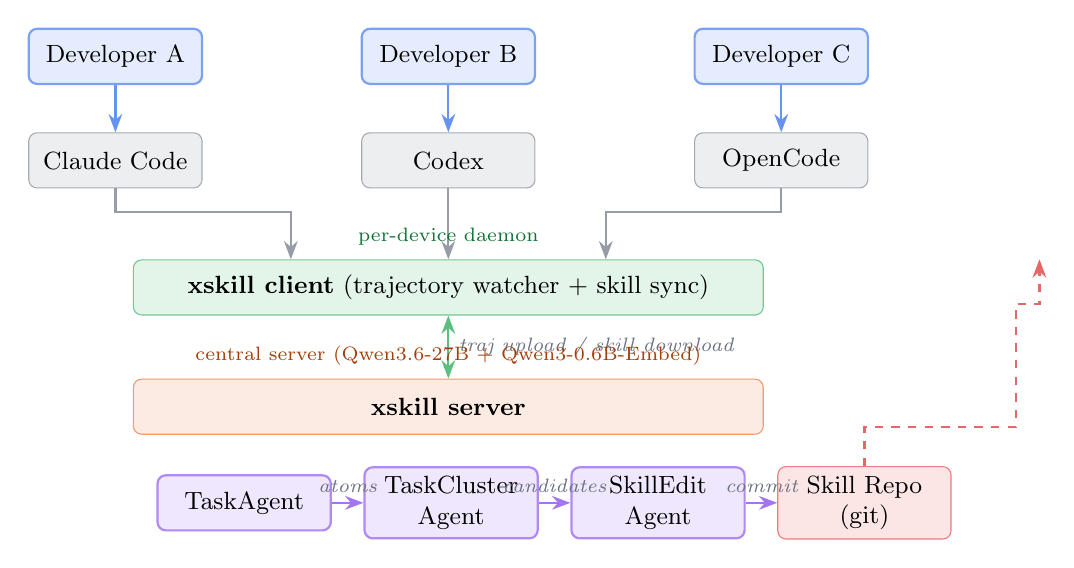
\begin{tikzpicture}[
    >=Stealth,
    node distance=0.6cm and 1.2cm,
    block/.style={rectangle, draw, rounded corners=3pt, minimum height=0.7cm, minimum width=2.2cm, font=\small, align=center, fill=#1!12, draw=#1!60},
    agent/.style={block=#1, thick},
    pipe/.style={->, thick, color=#1!70},
    label/.style={font=\scriptsize\itshape, color=xgray},
]

% --- User layer ---
\node[agent=xblue] (user1) {Developer A};
\node[agent=xblue, right=2.0cm of user1] (user2) {Developer B};
\node[agent=xblue, right=2.0cm of user2] (user3) {Developer C};

% --- Agent runtimes ---
\node[block=xgray, below=0.6cm of user1] (cc) {Claude Code};
\node[block=xgray, below=0.6cm of user2] (codex) {Codex};
\node[block=xgray, below=0.6cm of user3] (oc) {OpenCode};

% --- xskill client ---
\node[block=xgreen, below=0.9cm of codex, minimum width=8cm] (client) {\textbf{xskill client} (trajectory watcher + skill sync)};

% --- xskill server ---
\node[block=xorange, below=0.8cm of client, minimum width=8cm] (server) {\textbf{xskill server}};

% --- Three agents inside server ---
\node[agent=xpurple, below=0.5cm of server.south west, anchor=north west, xshift=0.3cm] (ta) {TaskAgent};
\node[agent=xpurple, right=0.4cm of ta] (tca) {TaskCluster\\Agent};
\node[agent=xpurple, right=0.4cm of tca] (sea) {SkillEdit\\Agent};

% --- Skill repo ---
\node[block=xred, right=0.4cm of sea] (repo) {Skill Repo\\(git)};

% --- Arrows: users to agents ---
\draw[pipe=xblue] (user1) -- (cc);
\draw[pipe=xblue] (user2) -- (codex);
\draw[pipe=xblue] (user3) -- (oc);

% --- Arrows: agents to client ---
\draw[pipe=xgray] (cc.south) -- ++(0,-0.3) -| ([xshift=-2cm]client.north);
\draw[pipe=xgray] (codex.south) -- (client.north);
\draw[pipe=xgray] (oc.south) -- ++(0,-0.3) -| ([xshift=2cm]client.north);

% --- Client to server ---
\draw[pipe=xgreen, <->] (client.south) -- node[right, label] {traj upload / skill download} (server.north);

% --- Server internal flow ---
\draw[pipe=xpurple] (ta.east) -- node[above, label] {atoms} (tca.west);
\draw[pipe=xpurple] (tca.east) -- node[above, label] {candidates} (sea.west);
\draw[pipe=xpurple] (sea.east) -- node[above, label] {commit} (repo.west);

% --- Skill back to client ---
\draw[pipe=xred, dashed, thick] (repo.north) -- ++(0,0.5) -| ([xshift=3.2cm]server.north east) -- ++(0,0.95) -| ([xshift=3.5cm]client.north east);

% --- Labels ---
\node[above=0.05cm of client, font=\scriptsize\color{xgreen!70!black}] {per-device daemon};
\node[above=0.05cm of server, font=\scriptsize\color{xorange!70!black}] {central server (Qwen3.6-27B + Qwen3-0.6B-Embed)};

\end{tikzpicture}
\caption{\textbf{xskill system overview.} Developers use their preferred coding agents (Claude Code, Codex, OpenCode, etc.). The xskill client daemon watches trajectory directories and uploads sanitized deltas to the central server. The server's three-agent pipeline decomposes trajectories into atomic tasks, clusters them into skill candidates, and produces versioned SKILL.md artifacts via git commits. Evolved skills are synced back to each developer's agent runtime.}
\label{fig:overview}
\end{figure}

We present \textbf{xskill}, an open-source system that addresses all three challenges. xskill operates as a \emph{management layer} above existing coding-agent runtimes (Figure~\ref{fig:overview}). It does not replace any agent's skill loader; instead, it shapes what those loaders read from disk. The key insight is that the \emph{lifecycle} of a skill---creation, evaluation, evolution, retirement---is orthogonal to the \emph{runtime} that loads and injects skills into agent prompts, and should therefore be managed by a dedicated system.

Our contributions are:
\begin{enumerate}
    \item A \textbf{cross-agent trajectory collection} architecture supporting 5 coding-agent ecosystems (Claude Code, Codex, OpenCode, OpenClaw, Hermes) through a unified normalizer interface.
    \item A \textbf{three-agent pipeline} (TaskAgent $\to$ TaskClusterAgent $\to$ SkillEditAgent) for automatic skill distillation from raw trajectories, with cumulative evidence thresholds replacing single-trajectory heuristics.
    \item A \textbf{canary evaluation protocol} using git branching (staging vs.\ main) and UX scoring---the first such mechanism in the trajectory-to-skill literature.
    \item A \textbf{comprehensive survey} of 10 trajectory-to-skill systems across 5 design dimensions (trigger, storage, production, evaluation, usage), providing the first systematic comparison matrix for this emerging field.
\end{enumerate}

%============================================================================
\section{Related Work}
\label{sec:related}
%============================================================================

We surveyed 10 systems that convert agent trajectories or experiences into reusable procedural knowledge. Table~\ref{tab:landscape} presents the landscape overview; here we discuss the most instructive comparisons.

\begin{table}[t]
\centering
\caption{\textbf{Landscape of trajectory-to-skill systems.} Columns indicate whether the system produces SKILL.md files, supports online (per-turn) triggering, implements deduplication, performs canary/A-B evaluation, and targets production coding-agent deployment.}
\label{tab:landscape}
\small
\begin{tabular}{@{}lccccc@{}}
\toprule
\textbf{System} & \textbf{SKILL.md} & \textbf{Online} & \textbf{Dedup} & \textbf{Canary} & \textbf{Production} \\
\midrule
OpenSpace      & \checkmark & \checkmark & \checkmark & $\times$ & \checkmark \\
EvoSkill       & \checkmark & $\times$   & $\times$   & $\times$ & \checkmark \\
AutoSkill      & \checkmark & \checkmark & \checkmark & $\times$ & \checkmark \\
Hermes         & \checkmark & $\times$   & $\times$   & $\times$ & $\times$ \\
GEPA-gskill    & \checkmark & $\times$   & $\times$   & $\times$ & $\times$ \\
Trace2Skill    & $\times$   & $\times$   & $\times$   & $\times$ & $\times$ \\
AgentEvolver   & $\times$   & $\times$   & $\times$   & $\times$ & $\times$ \\
MemSkill       & $\times$   & $\times$   & $\times$   & $\times$ & $\times$ \\
EvoAgentX      & $\times$   & $\times$   & $\times$   & $\times$ & $\times$ \\
SE-Agent       & $\times$   & $\times$   & $\times$   & $\times$ & $\times$ \\
SkillRL        & $\times$   & $\times$   & $\times$   & $\times$ & $\times$ \\
\midrule
\textbf{xskill} & \checkmark & \checkmark & \checkmark & \checkmark & \checkmark \\
\bottomrule
\end{tabular}
\end{table}

\subsection{Skill-as-SKILL.md Systems}

\textbf{OpenSpace}~\citep{hku2025openspace} is the closest system to xskill in scope. It maintains an evolving skill library via an MCP server, with three evolution triggers (per-task analysis, tool-degradation events, and periodic counters) feeding into a 3$\times$3 evolution type matrix (FIX / DERIVED / CAPTURED). However, OpenSpace wraps skill execution inside its own sub-agent---meaning the host agent's harness (e.g., \texttt{CLAUDE.md} rules) does not apply during skill-enhanced execution, a fundamental isolation problem for production use.

\textbf{EvoSkill}~\citep{sentient2025evoskill} uses git branches as program versions and Pareto frontiers for selection, offering the cleanest version-control story among all surveyed systems. However, it requires offline batch execution and does not support real-time trajectory collection.

\textbf{AutoSkill}~\citep{ecnu2025autoskill} is the only system besides xskill that achieves per-turn asynchronous skill extraction during live chat. Its three-layer deduplication sandwich (identity hash $\to$ semantic+BM25 $\to$ LLM judge) is the most sophisticated deduplication mechanism we found. However, AutoSkill operates as a standalone framework rather than integrating with existing agent ecosystems.

\subsection{Non-SKILL.md Systems}

Several systems use alternative representations: \textbf{MemSkill}~\citep{memskill2025} uses RL-trained PPO controllers over operation banks; \textbf{EvoAgentX}~\citep{evoagentx2025} evolves workflow code; \textbf{SE-Agent}~\citep{seagent2025} replaces per-instance system prompts; \textbf{SkillRL}~\citep{skillrl2025} trains RL agents with JSON skill records; and \textbf{AgentEvolver}~\citep{agentevolver2025} delegates to an external ReMe memory service. These systems target RL training loops rather than production coding-agent deployments and are thus complementary to xskill's scope.

\textbf{Trace2Skill}~\citep{alibaba2025trace2skill} proposes a MapReduce-style patch merging approach and demonstrates that machine-generated skills can outperform human-written ones (on SpreadsheetBench). Its key finding---cross-model skill transfer is viable---supports xskill's design of centralized skill production that serves heterogeneous client runtimes.

\textbf{GEPA}~\citep{gepa2025} introduces system-aware three-way merge by common ancestor, analogous to git's merge algorithm applied to prompt evolution. This is the most principled merge mechanism we found, and xskill's git-based versioning enables similar ancestral reasoning.

\subsection{Key Gap: No System Does A/B Evaluation}

\begin{figure}[t]
\centering
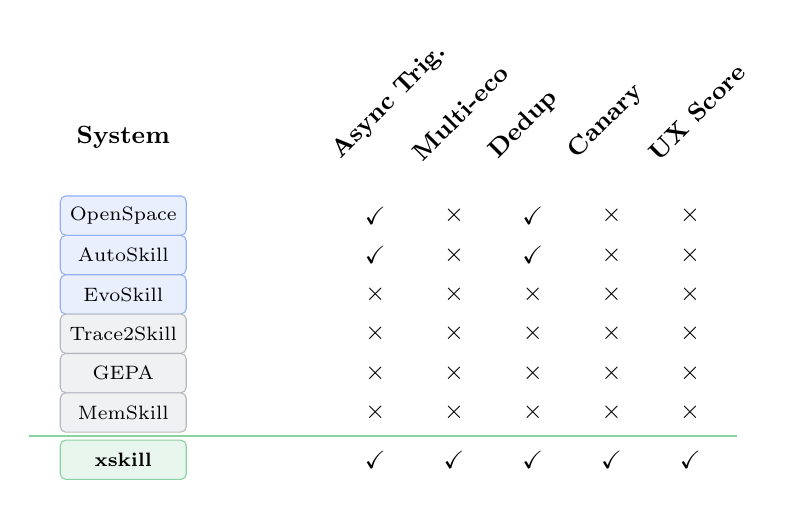
\begin{tikzpicture}[
    >=Stealth,
    sys/.style={rectangle, draw, rounded corners=2pt, minimum width=1.6cm, minimum height=0.5cm, font=\scriptsize, align=center, fill=#1!10, draw=#1!50},
    check/.style={font=\Large},
    cross/.style={font=\Large, color=xred!70},
]
% Column headers
\node[font=\small\bfseries] at (0, 3.8) {System};
\node[font=\small\bfseries, rotate=45, anchor=south west] at (2.8, 3.3) {Async Trig.};
\node[font=\small\bfseries, rotate=45, anchor=south west] at (3.8, 3.3) {Multi-eco};
\node[font=\small\bfseries, rotate=45, anchor=south west] at (4.8, 3.3) {Dedup};
\node[font=\small\bfseries, rotate=45, anchor=south west] at (5.8, 3.3) {Canary};
\node[font=\small\bfseries, rotate=45, anchor=south west] at (6.8, 3.3) {UX Score};

% Systems
\foreach \name/\y/\c/\a/\b/\d/\e/\f in {
    OpenSpace/2.8/xblue/\checkmark/$\times$/\checkmark/$\times$/$\times$,
    AutoSkill/2.3/xblue/\checkmark/$\times$/\checkmark/$\times$/$\times$,
    EvoSkill/1.8/xblue/$\times$/$\times$/$\times$/$\times$/$\times$,
    Trace2Skill/1.3/xgray/$\times$/$\times$/$\times$/$\times$/$\times$,
    GEPA/0.8/xgray/$\times$/$\times$/$\times$/$\times$/$\times$,
    MemSkill/0.3/xgray/$\times$/$\times$/$\times$/$\times$/$\times$,
    \textbf{xskill}/-0.3/xgreen/\checkmark/\checkmark/\checkmark/\checkmark/\checkmark%
} {
    \node[sys=\c] at (0, \y) {\name};
    \node[font=\small] at (3.2, \y) {\a};
    \node[font=\small] at (4.2, \y) {\b};
    \node[font=\small] at (5.2, \y) {\d};
    \node[font=\small] at (6.2, \y) {\e};
    \node[font=\small] at (7.2, \y) {\f};
}

% Separator line
\draw[thick, xgreen!50] (-1.2, 0.0) -- (7.8, 0.0);

\end{tikzpicture}
\caption{\textbf{Feature coverage of trajectory-to-skill systems} on five dimensions critical for team deployment. Only xskill covers all five: asynchronous per-turn triggering, multi-ecosystem support, deduplication, canary-based A/B testing, and user-experience scoring. None of the 10 surveyed systems implement canary or UX evaluation.}
\label{fig:features}
\end{figure}

Across all 10 surveyed systems, \emph{none} implements canary/A/B evaluation (Figure~\ref{fig:features}). Most evaluate skills via offline benchmarks (EvoSkill, GEPA, MemSkill) or LLM-as-judge on the skill text itself (OpenSpace). Only AutoSkill tracks per-turn \texttt{relevant/used} judgments via an LLM judge, but this measures skill selection quality, not downstream user experience. The absence of A/B testing means that skill evolution in all existing systems is driven by proxy metrics rather than direct evidence of user benefit---a gap xskill explicitly addresses.


%============================================================================
\section{System Architecture}
\label{sec:architecture}
%============================================================================

xskill consists of two components: a \textbf{client daemon} running on each developer's machine, and a \textbf{central server} that hosts the three-agent pipeline and the skill repository.

\subsection{Cross-Agent Trajectory Collection}
\label{sec:collection}

\begin{figure}[t]
\centering
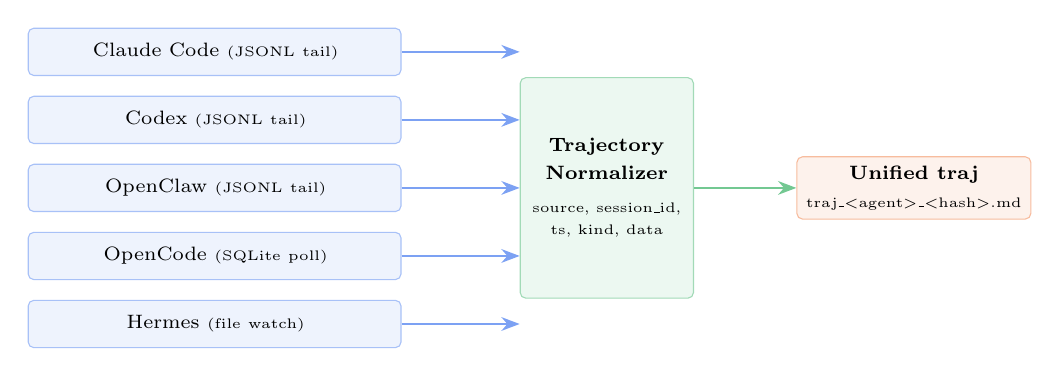
\begin{tikzpicture}[
    >=Stealth,
    node distance=0.4cm,
    src/.style={rectangle, draw, rounded corners=2pt, minimum height=0.6cm, font=\scriptsize, align=center, text width=4.5cm, fill=xblue!8, draw=xblue!40},
    norm/.style={rectangle, draw, rounded corners=2pt, minimum height=0.6cm, font=\scriptsize, align=center, fill=xgreen!8, draw=xgreen!40},
    outnode/.style={rectangle, draw, rounded corners=2pt, minimum height=0.6cm, font=\scriptsize, align=center, fill=xorange!8, draw=xorange!40},
]

% Sources
\node[src] (cc) {Claude Code {\tiny(JSONL tail)}};
\node[src, below=0.25cm of cc] (codex) {Codex {\tiny(JSONL tail)}};
\node[src, below=0.25cm of codex] (oclaw) {OpenClaw {\tiny(JSONL tail)}};
\node[src, below=0.25cm of oclaw] (ocode) {OpenCode {\tiny(SQLite poll)}};
\node[src, below=0.25cm of ocode] (hermes) {Hermes {\tiny(file watch)}};

% Normalizer
\node[norm, right=1.5cm of oclaw, minimum height=2.8cm, minimum width=2.2cm] (normalizer) {\textbf{Trajectory}\\[2pt]\textbf{Normalizer}\\[4pt]{\tiny source, session\_id,}\\{\tiny ts, kind, data}};

% Output
\node[outnode, right=1.3cm of normalizer, minimum width=2.5cm] (theoutput) {\textbf{Unified traj}\\[2pt]{\tiny traj\_<agent>\_<hash>.md}};

% Arrows
\draw[->, thick, xblue!60] (cc.east) -- (cc.east -| normalizer.west);
\draw[->, thick, xblue!60] (codex.east) -- (codex.east -| normalizer.west);
\draw[->, thick, xblue!60] (oclaw.east) -- (normalizer.west);
\draw[->, thick, xblue!60] (ocode.east) -- (ocode.east -| normalizer.west);
\draw[->, thick, xblue!60] (hermes.east) -- (hermes.east -| normalizer.west);
\draw[->, thick, xgreen!60] (normalizer.east) -- (theoutput.west);

\end{tikzpicture}
\caption{\textbf{Cross-agent trajectory collection.} Each coding agent writes trajectories in its native format and path. The xskill client runs per-agent adapters that normalize events into a unified schema. Four of five agents use appendable JSONL files, enabling efficient \texttt{inotify}/\texttt{tail} collection; OpenCode's SQLite database requires polling.}
\label{fig:collection}
\end{figure}

A key design decision is that xskill does \emph{not} require agents to push trajectories; instead, the client daemon \emph{pulls} from known filesystem locations (Figure~\ref{fig:collection}). This zero-configuration approach works because all five supported agents write trajectories to predictable paths:

\begin{itemize}
    \item \textbf{Claude Code}: \texttt{\~{}/.claude/projects/<proj>/<sid>.jsonl} --- JSONL, async batch append.
    \item \textbf{Codex}: \texttt{\~{}/.codex/sessions/YYYY/MM/DD/rollout-*.jsonl} --- JSONL, streaming append.
    \item \textbf{OpenClaw}: \texttt{\~{}/.openclaw/agents/<id>/sessions/*.trajectory.jsonl} --- JSONL, per-event sync.
    \item \textbf{OpenCode}: \texttt{\~{}/.local/share/opencode/opencode.db} --- SQLite (the only non-JSONL format).
    \item \textbf{Hermes}: \texttt{<cwd>/trajectory\_samples.jsonl} --- JSONL, written at run end.
\end{itemize}

Each trajectory event is normalized into a \texttt{TrajectoryEvent} schema with fields: \texttt{source} (agent identifier), \texttt{session\_id}, \texttt{ts} (ISO 8601), \texttt{kind} (user\_msg $|$ assistant\_msg $|$ tool\_call $|$ tool\_result $|$ session\_start $|$ session\_end $|$ compact), and \texttt{data} (native payload preserved for replay). The watcher scans registered directories every 30 seconds; new or appended content triggers the TaskAgent pipeline.

\paragraph{Sanitization.} Before upload, the client applies secret-pattern redaction (API keys, tokens, credentials) using a configurable regex set, ensuring that team-shared trajectories do not leak sensitive data.

\subsection{Three-Agent Pipeline}
\label{sec:pipeline}

\begin{figure}[t]
\centering
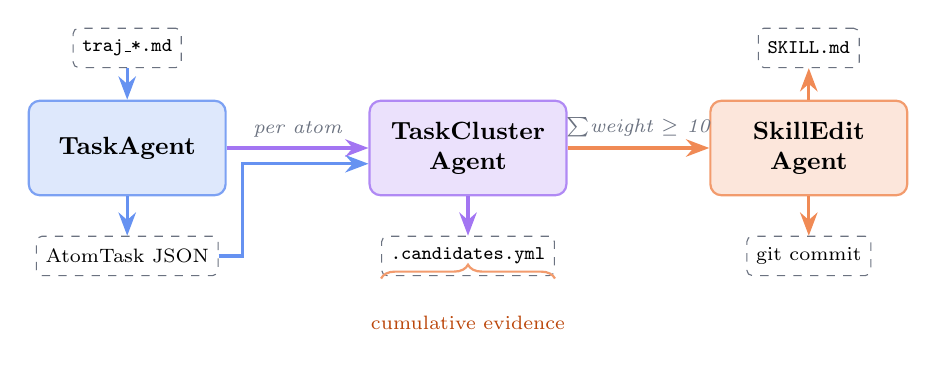
\begin{tikzpicture}[
    >=Stealth,
    node distance=0.8cm,
    stage/.style={rectangle, draw, rounded corners=4pt, minimum height=1.2cm, minimum width=2.5cm, font=\small\bfseries, align=center, fill=#1!15, draw=#1!60, thick},
    data/.style={rectangle, draw, dashed, rounded corners=2pt, minimum height=0.5cm, font=\scriptsize, fill=white, draw=xgray},
    arr/.style={->, very thick, color=#1!70},
]

% Stages
\node[stage=xblue] (ta) {TaskAgent};
\node[stage=xpurple, right=1.8cm of ta] (tca) {TaskCluster\\Agent};
\node[stage=xorange, right=1.8cm of tca] (sea) {SkillEdit\\Agent};

% Data nodes
\node[data, above=0.4cm of ta] (traj) {\texttt{traj\_*.md}};
\node[data, below=0.5cm of ta] (atoms) {AtomTask JSON};

\node[data, below=0.5cm of tca] (cands) {\texttt{.candidates.yml}};

\node[data, above=0.4cm of sea] (skillmd) {\texttt{SKILL.md}};
\node[data, below=0.5cm of sea] (git) {git commit};

% Arrows
\draw[arr=xblue] (traj) -- (ta);
\draw[arr=xblue] (ta) -- (atoms);
\draw[arr=xblue] (atoms.east) -- ++(0.3,0) |- ([yshift=-0.2cm]tca.west);

\draw[arr=xpurple] (ta.east) -- node[above, font=\scriptsize\itshape, color=xgray] {per atom} (tca.west);
\draw[arr=xpurple] (tca) -- (cands);

\draw[arr=xorange] (tca.east) -- node[above, font=\scriptsize\itshape, color=xgray] {$\sum$weight $\geq$ 10} (sea.west);
\draw[arr=xorange] (sea) -- (skillmd);
\draw[arr=xorange] (sea) -- (git);

% Threshold annotation
\draw[decorate, decoration={brace, amplitude=5pt, raise=2pt}, thick, xorange!60]
    ([yshift=-0.1cm]cands.south west) -- ([yshift=-0.1cm]cands.south east)
    node[midway, below=8pt, font=\scriptsize, color=xorange!80!black] {cumulative evidence};

\end{tikzpicture}
\caption{\textbf{Three-agent pipeline.} \emph{TaskAgent} decomposes trajectory deltas into AtomTask segments. \emph{TaskClusterAgent} routes each atom to an existing or new skill, appending weighted evidence. \emph{SkillEditAgent} fires when cumulative evidence exceeds a threshold (default: weight$\geq$10), producing or updating SKILL.md via git commit.}
\label{fig:pipeline}
\end{figure}

The server processes normalized trajectories through three specialized agents (Figure~\ref{fig:pipeline}):

\subsubsection{TaskAgent: Trajectory Decomposition}

Raw trajectories are multi-topic conversations that may span hours. The TaskAgent segments each trajectory into \textbf{AtomTasks}---coherent units representing a single user intent (e.g., ``deploy FastAPI to port 1717'' or ``fix the SQLite migration''). Each AtomTask records:

\begin{itemize}
    \item \texttt{atom\_id}: unique identifier (\texttt{atom\_<traj\_id>\_NNNN})
    \item \texttt{intent}, \texttt{summary}, \texttt{tags}: semantic metadata
    \item \texttt{used\_skills}: skills the agent self-reported using
    \item \texttt{ux\_score}: user-experience score ($0$--$10$), used in canary evaluation
    \item \texttt{offset\_start}, \texttt{offset\_end}: character offsets for provenance
    \item \texttt{pre\_atom\_id}, \texttt{post\_atom\_id}: linked-list neighbors for context
\end{itemize}

The UX score is assigned by the TaskAgent based on signals such as: whether the user accepted the agent's output, whether corrections were needed, and whether the session segment ended naturally or was abandoned.

\subsubsection{TaskClusterAgent: Skill Routing}

Each AtomTask triggers a TaskClusterAgent (TCA) invocation. The TCA receives the atom plus a catalog of existing skills (name + truncated description) and makes one of three decisions:

\begin{enumerate}
    \item \textbf{Route to existing skill}: append the atom to the skill's \texttt{.candidates.yml} with a \texttt{weightscore} (0--10) reflecting the atom's relevance.
    \item \textbf{Create new skill}: initialize a new skill folder in ``baby'' state with the atom as its first evidence.
    \item \textbf{Reclassify}: move an atom from one skill to another if the TCA determines a better fit.
\end{enumerate}

The TCA's routing is LLM-based but constrained by the existing catalog structure, preventing unbounded skill proliferation while allowing organic growth.

\subsubsection{SkillEditAgent: Skill Production}

When a skill's \texttt{.candidates.yml} accumulates a cumulative \texttt{weightscore} $\geq \theta$ (default $\theta = 10$), the SkillEditAgent (SEA) fires. The SEA reads all candidate atoms (via \texttt{AtomTaskRead}), optionally reads raw trajectory text (via \texttt{ReadTraj}), and produces or updates the skill's \texttt{SKILL.md} along with any auxiliary files (scripts, references).

The SEA's commit behavior depends on branch state:
\begin{itemize}
    \item \textbf{Baby branch $\to$ main}: first public version of a new skill.
    \item \textbf{Main branch $\to$ staging}: creates a canary candidate for A/B comparison.
\end{itemize}

This branching model ensures that skill updates are never applied directly to main without canary evaluation.

\subsection{Canary Evaluation Protocol}
\label{sec:canary}

\begin{figure}[t]
\centering
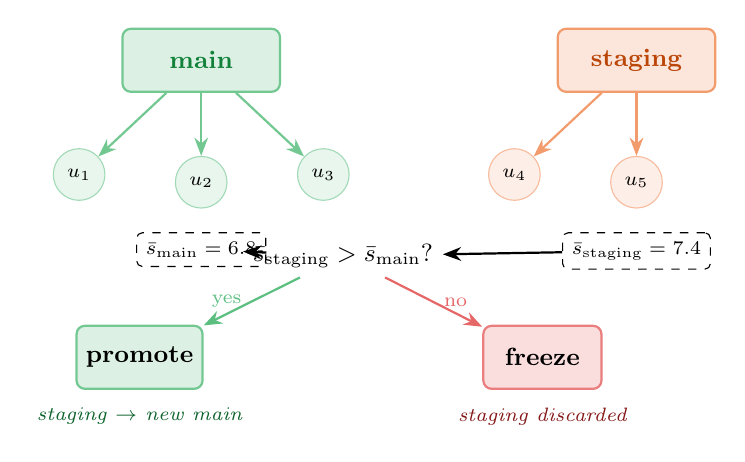
\begin{tikzpicture}[
    >=Stealth,
    node distance=0.5cm and 1.0cm,
    branch/.style={rectangle, draw, rounded corners=3pt, minimum height=0.8cm, minimum width=2.0cm, font=\small\bfseries, fill=#1!15, draw=#1!60, thick},
    user/.style={circle, draw, minimum size=0.6cm, font=\scriptsize, fill=#1!10, draw=#1!40},
    score/.style={rectangle, draw, dashed, rounded corners=2pt, font=\scriptsize, fill=white},
]

% Branches
\node[branch=xgreen] (main) {\textcolor{xgreen!80!black}{main}};
\node[branch=xorange, right=3.5cm of main] (staging) {\textcolor{xorange!80!black}{staging}};

% Users under main
\node[user=xgreen, below left=0.8cm and 0.3cm of main] (u1) {$u_1$};
\node[user=xgreen, below=0.8cm of main] (u2) {$u_2$};
\node[user=xgreen, below right=0.8cm and 0.3cm of main] (u3) {$u_3$};

% Users under staging
\node[user=xorange, below left=0.8cm and 0.3cm of staging] (u4) {$u_4$};
\node[user=xorange, below=0.8cm of staging] (u5) {$u_5$};

% Arrows
\draw[->, thick, xgreen!60] (main) -- (u1);
\draw[->, thick, xgreen!60] (main) -- (u2);
\draw[->, thick, xgreen!60] (main) -- (u3);
\draw[->, thick, xorange!60] (staging) -- (u4);
\draw[->, thick, xorange!60] (staging) -- (u5);

% UX scores
\node[score, below=0.3cm of u2] (sm) {$\bar{s}_{\text{main}} = 6.8$};
\node[score, below=0.3cm of u5] (ss) {$\bar{s}_{\text{staging}} = 7.4$};

% Decision
\node[font=\small, below=1.8cm of main, xshift=1.8cm] (decision) {$\bar{s}_{\text{staging}} > \bar{s}_{\text{main}}$?};

% Outcomes
\node[branch=xgreen, below left=0.6cm and 0.5cm of decision, minimum width=1.5cm] (promote) {promote};
\node[branch=xred, below right=0.6cm and 0.5cm of decision, minimum width=1.5cm] (freeze) {freeze};

\draw[->, thick] (sm) -- (decision);
\draw[->, thick] (ss) -- (decision);
\draw[->, thick, xgreen!70] (decision) -- node[left, font=\scriptsize] {yes} (promote);
\draw[->, thick, xred!70] (decision) -- node[right, font=\scriptsize] {no} (freeze);

% Promote annotation
\node[font=\scriptsize\itshape, color=xgreen!60!black, below=0.1cm of promote] {staging $\to$ new main};
\node[font=\scriptsize\itshape, color=xred!60!black, below=0.1cm of freeze] {staging discarded};

\end{tikzpicture}
\caption{\textbf{Canary evaluation protocol.} When the SkillEditAgent produces an updated skill, it commits to a staging branch. The xskill server routes a subset of users ($u_4, u_5$) to the staging version while the majority ($u_1, u_2, u_3$) continue on main. UX scores from AtomTasks using each branch are aggregated; the staging branch is promoted to main only if its mean score exceeds main's.}
\label{fig:canary}
\end{figure}

The canary protocol (Figure~\ref{fig:canary}) is xskill's primary quality gate. When a SkillEditAgent commits an updated skill to a staging branch, the system:

\begin{enumerate}
    \item \textbf{Maintains a single active canary per skill}: new candidates queue rather than overwriting, preventing evaluation contamination.
    \item \textbf{Routes a configurable fraction} of users to the staging version (via skill file sync to their machines).
    \item \textbf{Collects UX scores} from AtomTasks that use the skill under both branches. Each score $s \in [0, 10]$ is attributed to the branch (\texttt{side=main} or \texttt{side=staging}) under which it was observed.
    \item \textbf{Evaluates}: when sufficient samples accumulate, compares $\bar{s}_{\text{staging}}$ vs.\ $\bar{s}_{\text{main}}$. If staging wins, it replaces main; otherwise, it is frozen (retained for audit, hidden from runtime).
\end{enumerate}

The UX score is \emph{not} an LLM self-evaluation. It is derived from observable behavioral signals: task completion, absence of user corrections, natural session transitions. This distinguishes xskill's evaluation from the LLM-as-judge approaches used by OpenSpace and AutoSkill.

\subsection{Cross-Agent Skill Distribution}
\label{sec:distribution}

\begin{table}[t]
\centering
\caption{\textbf{Skill output paths for 5 agent ecosystems.} The SKILL.md format with YAML frontmatter (\texttt{name} + \texttt{description}) is the cross-agent interoperability unit. Two filesystem paths---\texttt{\~{}/.claude/skills/} and \texttt{\~{}/.agents/skills/}---cover 4 of 5 ecosystems; only Hermes requires a dedicated path.}
\label{tab:distribution}
\small
\begin{tabular}{@{}lll@{}}
\toprule
\textbf{Agent Ecosystem} & \textbf{xskill Output Path} & \textbf{Also Scanned By} \\
\midrule
Claude Code & \texttt{\~{}/.claude/skills/<name>/SKILL.md} & OpenCode \\
Codex       & \texttt{\~{}/.agents/skills/<name>/SKILL.md} & OpenClaw \\
OpenCode    & \texttt{\~{}/.claude/skills/<name>/SKILL.md} & Claude Code \\
OpenClaw    & \texttt{\~{}/.agents/skills/<name>/SKILL.md} & Codex \\
Hermes      & \texttt{\~{}/.hermes/skills/<cat>/<name>/SKILL.md} & (exclusive) \\
\bottomrule
\end{tabular}
\end{table}

A critical finding from our ecosystem survey is that \textbf{SKILL.md with YAML frontmatter is the de facto cross-agent standard}. Five of the ten surveyed systems produce this format, and all five supported agent runtimes parse it. Table~\ref{tab:distribution} shows xskill's output path strategy.

The frontmatter uses a compatible superset:
\begin{verbatim}
---
name: <slug>
description: <one-line, <=1024 chars>
version: 1.0.0
metadata:
  hermes: {tags: [...]}
  openclaw: {emoji: "...", requires: {...}}
  short-description: <Codex alias>
---
\end{verbatim}
Private fields are silently ignored by non-target runtimes (all five do YAML-tolerant parsing), so a single artifact serves all ecosystems.


%============================================================================
\section{Design Dimensions: A Comparative Analysis}
\label{sec:dimensions}
%============================================================================

Our survey organizes the trajectory-to-skill landscape into five dimensions. We present key findings per dimension, positioning xskill's choices.

\subsection{Trigger Mechanism}

\begin{table}[t]
\centering
\caption{\textbf{Trigger mechanisms across 10 systems + xskill.} ``Async'' = non-blocking; ``Per-turn'' = can fire during a live conversation; ``User-transparent'' = the user does not explicitly request skill generation.}
\label{tab:trigger}
\small
\begin{tabular}{@{}lcccl@{}}
\toprule
\textbf{System} & \textbf{Async} & \textbf{Per-turn} & \textbf{Transparent} & \textbf{Mechanism} \\
\midrule
Hermes         & -- & -- & -- & Offline CLI \\
OpenSpace      & \checkmark & \checkmark & \checkmark & Hook + counter + event \\
EvoSkill       & -- & -- & -- & Offline batch \\
AutoSkill      & \checkmark & \checkmark & \checkmark & Per-turn + background thread \\
AgentEvolver   & -- & -- & -- & Counter in RL loop \\
MemSkill       & -- & -- & -- & Counter in RL loop \\
EvoAgentX      & -- & -- & -- & Offline batch loop \\
SE-Agent       & -- & -- & -- & Offline iteration \\
SkillRL        & -- & -- & -- & Counter + success gate \\
GEPA           & -- & -- & -- & Offline batch \\
\midrule
\textbf{xskill} & \checkmark & \checkmark & \checkmark & 30s watcher + per-atom async \\
\bottomrule
\end{tabular}
\end{table}

Eight of ten systems use offline batch or counter-based triggers (Table~\ref{tab:trigger}). Only OpenSpace and AutoSkill achieve user-transparent, per-turn triggering. xskill adopts a 30-second polling watcher with per-atom asynchronous processing, achieving transparency without requiring hook registration in the host agent (though hooks can accelerate detection when available).

\subsection{Skill Production}

All 10 systems use LLM-as-author for skill text generation---no system attempts rule-based, template, or AST-based production. xskill follows this pattern but adds \emph{cumulative evidence}: rather than generating a skill from a single trajectory, the SkillEditAgent waits for multiple weighted atoms to accumulate, reducing the risk of overfitting to a single interaction.

\subsection{Deduplication and Merging}

Deduplication maturity varies enormously: from zero (Hermes, SE-Agent, EvoAgentX) to AutoSkill's six-layer sandwich. xskill's TCA performs catalog-aware routing (LLM judgment over existing skill names and descriptions), which provides moderate deduplication without the complexity of AutoSkill's multi-stage pipeline.

\subsection{Evaluation and Retirement}

Most systems evaluate skills via offline benchmarks or LLM self-judgment. The ``only increase, never delete'' pattern is dominant (7/10 systems). xskill introduces canary evaluation (\S\ref{sec:canary}) and supports skill freezing (retained for audit, removed from active distribution).

\subsection{Skill Injection}

\begin{table}[t]
\centering
\caption{\textbf{Skill injection strategies.} xskill does not inject skills itself---it publishes to disk, and the host runtime's loader handles injection. This decoupling is deliberate: it preserves each runtime's native caching, trimming, and compaction behavior.}
\label{tab:injection}
\small
\begin{tabular}{@{}ll@{}}
\toprule
\textbf{Strategy} & \textbf{Systems} \\
\midrule
Full body in system prompt & OpenSpace, AutoSkill, MemSkill, SE-Agent, SkillRL \\
Directory listing + Read tool & Codex, OpenClaw \\
CLI autodiscovery (no injection) & EvoSkill \\
User message injection & AgentEvolver \\
\textbf{Publish to disk (runtime-agnostic)} & \textbf{xskill}, GEPA-gskill \\
\bottomrule
\end{tabular}
\end{table}

xskill deliberately avoids injecting skills into agent prompts (Table~\ref{tab:injection}). Instead, it publishes SKILL.md files to the directories each runtime already scans. This preserves native behaviors: Claude Code's 1\% listing budget and compaction, Codex's progressive disclosure, OpenCode's full-dump strategy. The management layer shapes \emph{what} is available; the runtime decides \emph{how} to present it.

%============================================================================
\section{Discussion}
\label{sec:discussion}
%============================================================================

\subsection{Design Trade-offs}

\paragraph{Pull vs.\ Push trajectory collection.} xskill pulls from known paths rather than requiring agents to push events. This trades real-time latency (30s polling vs.\ sub-second hooks) for zero-configuration deployment. For Claude Code and Codex, hooks can be registered to reduce latency; the pull mechanism serves as a universal fallback.

\paragraph{Cumulative evidence vs.\ single-trajectory skill creation.} Most systems (OpenSpace, AutoSkill, SE-Agent) can create a skill from a single trajectory. xskill requires cumulative weighted evidence ($\geq\theta$), which delays skill creation but reduces noise. This is especially important in team settings where trajectory quality varies across developers.

\paragraph{UX scoring vs.\ LLM judging.} xskill's UX scores are derived from behavioral signals (task completion, user corrections) rather than LLM self-evaluation. This avoids the well-documented biases of LLM-as-judge~\citep{zheng2024judging} at the cost of noisier signals.

\subsection{Limitations}

\begin{enumerate}
    \item \textbf{No formal evaluation}: xskill is an engineering system deployed in team settings, not a controlled experiment. We do not report pass@1 numbers on standardized benchmarks because the system targets real-world skill evolution rather than isolated task completion.
    \item \textbf{Model dependency}: the server's three-agent pipeline currently requires Qwen3.6-27B for generation and Qwen3-0.6B-Embed for embeddings. The minimum hardware is a single GPU server with $\geq$40GB VRAM.
    \item \textbf{Cold start}: a new deployment begins with an empty skill repository. While xskill supports batch trajectory import for cold start, the canary mechanism requires ongoing user traffic to function.
    \item \textbf{OpenCode adapter}: OpenCode's SQLite-only trajectory storage makes it the most expensive ecosystem to integrate, requiring either plugin development or database polling.
\end{enumerate}

\subsection{Broader Impact}

xskill's team-level skill sharing raises questions about intellectual property and knowledge attribution. The sanitization pipeline strips secrets but does not address the subtler issue of whether automated skill distillation from one developer's work creates implicit IP obligations. Organizations deploying xskill should establish clear policies about skill ownership and attribution.

%============================================================================
\section{Conclusion}
\label{sec:conclusion}
%============================================================================

We presented xskill, a system for automatic skill distillation, team-level sharing, and data-driven evolution for coding agents. Through a comprehensive survey of 10 trajectory-to-skill systems, we identified that no existing system combines asynchronous cross-agent trajectory collection, cumulative-evidence skill production, canary-based A/B evaluation, and multi-ecosystem distribution. xskill fills this gap by operating as a management layer above existing coding-agent runtimes, shaping the skill supply without interfering with each runtime's native loading and injection mechanisms.

The emerging consensus on SKILL.md as a cross-agent interoperability format, combined with the predictable filesystem layout of modern coding agents, makes this management-layer architecture both practical and timely. As coding agents become standard development tools, the ability to systematically capture, evaluate, and distribute procedural knowledge across teams will be a critical differentiator. xskill is open-source at \url{https://github.com/SkillNerds/xskill}.

%============================================================================
% References
%============================================================================

\bibliographystyle{plainnat}

\begin{thebibliography}{20}

\bibitem[Anthropic(2025)]{anthropic2025claude}
Anthropic.
\newblock Claude Code: An agentic coding tool.
\newblock \url{https://claude.com/claude-code}, 2025.

\bibitem[OpenAI(2025)]{openai2025codex}
OpenAI.
\newblock Codex CLI: Lightweight coding agent.
\newblock \url{https://github.com/openai/codex}, 2025.

\bibitem[SST(2025)]{sst2025opencode}
SST.
\newblock OpenCode: Open-source coding agent.
\newblock \url{https://github.com/sst/opencode}, 2025.

\bibitem[Chen et~al.(2025)]{hku2025openspace}
Chen, Y., et~al.
\newblock OpenSpace: An evolving skill library via MCP for code agents.
\newblock \url{https://github.com/HKUDS/OpenSpace}, 2025.

\bibitem[Wang et~al.(2025)]{sentient2025evoskill}
Wang, J., et~al.
\newblock EvoSkill: Evolutionary program synthesis for agent skills.
\newblock \url{https://github.com/sentient-agi/EvoSkill}, 2025.

\bibitem[Li et~al.(2025)]{ecnu2025autoskill}
Li, X., et~al.
\newblock AutoSkill: Automated skill management for coding agents.
\newblock \url{https://github.com/ECNU-ICALK/AutoSkill}, 2025.

\bibitem[Qwen(2025)]{alibaba2025trace2skill}
Qwen Applications.
\newblock Trace2Skill: From agent traces to reusable skills.
\newblock \url{https://github.com/Qwen-Applications/Trace2Skill}, 2025.

\bibitem[ModelScope(2025)]{agentevolver2025}
ModelScope.
\newblock AgentEvolver: Evolving agents with reinforcement learning.
\newblock \url{https://github.com/modelscope/AgentEvolver}, 2025.

\bibitem[Axelsen(2025)]{memskill2025}
Axelsen, V.
\newblock MemSkill: Memory-augmented skill learning.
\newblock \url{https://github.com/ViktorAxelsen/MemSkill}, 2025.

\bibitem[EvoAgentX(2025)]{evoagentx2025}
EvoAgentX Team.
\newblock EvoAgentX: Evolutionary agent workflow optimization.
\newblock \url{https://github.com/EvoAgentX/EvoAgentX}, 2025.

\bibitem[Xu et~al.(2025)]{seagent2025}
Xu, S., et~al.
\newblock SE-Agent: Self-evolving agents for software engineering.
\newblock \url{https://github.com/JARVIS-Xs/SE-Agent}, 2025.

\bibitem[Aiming Lab(2025)]{skillrl2025}
Aiming Lab.
\newblock SkillRL: Skill-augmented reinforcement learning for agents.
\newblock \url{https://github.com/aiming-lab/SkillRL}, 2025.

\bibitem[GEPA(2025)]{gepa2025}
GEPA Team.
\newblock GEPA: Generalized evolutionary prompt optimization.
\newblock \emph{arXiv preprint arXiv:2507.19457}, 2025.

\bibitem[Zheng et~al.(2024)]{zheng2024judging}
Zheng, L., Chiang, W.-L., Sheng, Y., Zhuang, S., Wu, Z., Zhuang, Y., Lin, Z., Li, Z., Li, D., Xing, E.~P., et~al.
\newblock Judging {LLM}-as-a-Judge with {MT}-Bench and Chatbot Arena.
\newblock In \emph{NeurIPS}, 2024.

\end{thebibliography}

%============================================================================
% Appendix
%============================================================================
\newpage
\appendix

\section{Full Comparison Matrix}
\label{app:matrix}

\begin{table}[h!]
\centering
\caption{\textbf{Cross-system comparison on ``skill'' definition.} The term ``skill'' refers to fundamentally different artifacts across systems, complicating direct comparison.}
\label{tab:skill-def}
\small
\begin{tabular}{@{}llp{6cm}@{}}
\toprule
\textbf{\#} & \textbf{System} & \textbf{``Skill'' Artifact} \\
\midrule
1 & Hermes & Existing SKILL.md body (mutated in place) \\
2 & OpenSpace & Directory: SKILL.md + scripts/ + references/ + SQLite lineage \\
3 & EvoSkill & \texttt{.claude/skills/<name>/SKILL.md} (YAML frontmatter) \\
4 & AutoSkill & Per-user SKILL.md with semantic semver patches \\
5 & AgentEvolver & Vector-store entry in external ReMe service \\
6 & MemSkill & RL operation (INSERT/UPDATE/DELETE template) \\
7 & EvoAgentX & Workflow code: \texttt{round\_N/\{graph.py, prompt.py\}} \\
8 & SE-Agent & Per-instance system-prompt YAML \\
9 & SkillRL & JSON record: \texttt{\{title, principle, when\_to\_apply\}} \\
10 & GEPA & Candidate dict[str,str] (arbitrary optimizable text) \\
\midrule
11 & \textbf{xskill} & SKILL.md + auxiliary files, git-versioned, canary-evaluated \\
\bottomrule
\end{tabular}
\end{table}

\section{AtomTask Schema}
\label{app:atomtask}

\begin{verbatim}
{
  "atom_id": "atom_traj_cc_dsv4_890da9d9_0001",
  "traj_id": "traj_cc_dsv4_890da9d9",
  "offset_start": 120,
  "offset_end": 2400,
  "intent": "deploy xquiz on port 1717",
  "summary": "agent cloned repo, read README, configured port, started",
  "tags": ["deploy", "fastapi"],
  "used_skills": ["python-deploy"],
  "ux_score": 7,
  "pre_atom_id": null,
  "post_atom_id": "atom_traj_cc_dsv4_890da9d9_0002",
  "context_prefix": "",
  "raw_segment": ""
}
\end{verbatim}

\section{Canary Guard Conditions}
\label{app:canary-guards}

The SkillEditAgent is guarded by three conditions before committing to a staging branch:
\begin{enumerate}
    \item No staging branch currently exists for this skill (one canary at a time; new candidates queue).
    \item Cumulative \texttt{weightscore} of candidates $\geq \theta$ (default 10).
    \item If on main branch: at least one real \texttt{side=main} UX score exists (proves the current main version has been used, establishing a baseline for comparison).
\end{enumerate}

These guards prevent evaluation contamination from concurrent canaries and ensure that staging branches compete against a used---not merely published---main version.

\end{document}
